\documentclass{article}
\usepackage{enumitem}
\usepackage{indentfirst}
\usepackage{listings}
\usepackage{graphicx}
\usepackage{caption}
\usepackage[a4paper,portrait,margin=1in]{geometry}
%\pagenumbering{gobble}

\title{Tramway Code ltd. Employment exam}
\author{Svelte front-end engineer}
\begin{document}
\maketitle

\footnotetext[1]{The order doesn't matter, i.e. [1, 2] and [2, 1] are the same thing, and count as one single pair}
\footnotetext[2]{The position in the first array parameter, starting with 1}
\footnotetext[3]{The position in the second array parameter, starting with 1}

\section*{Exercise 1 (30 points)}
Let there be $N$ cities, from $1$ to $N$ in a cartesian coordinate system with known coordinates, and $M$ people, from $1$ to $M$, which have been in some cities.
We know for each of the $M$ people the cities they'be been in.
You will have to solve the following tasks:
\begin{enumerate}[label=\alph*)]
	\item For $C$ pairs of cities, find out the floor of the distance between the cities of each pair.
	\item Find out the pair of cities that are closest to each other.
	\item For $P$ pairs of people, find out the number of cities that both members of each pair have visited.
	\item Find out the number of pairs of people\footnotemark[1] which haven't any common visited city.
\end{enumerate}

You will have to write a JavaScript file which has as its default export a function that has 4 parameters:
\begin{enumerate}
	\item The first one is an array that contains $N$ arrays with exactly 2 numbers that describe a city, the first one being the $x$ coordinate, and the second one being the $y$ coordinate.
	\item The second one is an array that contains $M$ arrays which list, in the increasing order of their IDs\footnotemark[2], the cities visited by each person.
	\item The third one is an array that contains $C$ arrays with exactly 2 numbers representing, in the increasing order of their IDs\footnotemark[2] (position in the first array, starting at 1), the 2 cities whose distance has to be calculated.
	\item The fourth one is an array that contains $P$ arrays with exactly 2 numbers representing, in the increasing order of their IDs\footnotemark[3] (position in the second array, starting at 1), the 2 people whose number of cities visited by both has to be calculated.
\end{enumerate}

The function will return an object with the following contents:
\begin{itemize}
	\item \verb|answer_a|: an array with $C$ elements, each representing the floor of the distance of each pair of cites described in the third argument, in order.
	\item \verb|answer_b|: an array with 2 elements representing the IDs\footnotemark[2] of the 2 cites with the lowest distance. The order doesn't matter. If there are more possible answers, any one is OK.
	\item \verb|answer_c|: an array with $P$ elements, each representing for each pair the number of cities visited by both people.
	\item \verb|answer_d|: an integer representing the number of pairs of people\footnotemark[1] that don't share any visited city.
\end{itemize}

\subsection*{Procedure}
You shall clone in your workstation the git repository at \verb|https://10.192.192.19/ex1_|\fbox{ID}\verb|.git|, where \fbox{ID} is your given contestant ID.
There you should find an empty \verb|main.js| file. Write in it the function required by this problem, and push it in the remote whenever you feel like it.
This will trigger our CI to evaluate your sollution, and give you the score in the terminal right after pushing it. The best submission will give your score. Note that \textbf{you only have available 30 CI runs for this problem}.

\subsection*{Constraints}
\begin{itemize}
	\item \textbf{Time limit per test}: 1 second
	\item All the numbers involved in this exercise are integers.
	\item $1 < N, M < 10^4$
	\item $1 \leq C, P < 10^9$
	\item $-10^9 <$ any number of the first array parameter $< 10^9$
	\item $1 \leq$ any number of the second and third array parameters $\leq N$
	\item $1 \leq$ any number of the fourth array parameter $\leq M$
\end{itemize}

\subsection*{Example}
For the following given parameters:
\begin{enumerate}
	\item \verb|[[1, 3], [4, 3], [-1, -1]]|
	\item \verb|[[], [2], [1, 3], [1, 2]]|
	\item \verb|[[1, 2], [1, 3]]|
	\item \verb|[[1, 4], [2, 4], [2, 3]]|
\end{enumerate}

The function should return this object\footnote{Obviously, we're not reffering here to the \texttt{this} object}:
\begin{verbatim}
{
    answer_a: [3, 4],
    answer_b: [1, 2], // or [2, 1]
    answer_c: [0, 1, 0],
    answer_d: 4,
}
\end{verbatim}

\subsubsection*{Explanation}
\begin{figure}[h]
	\centering
	\begin{minipage}{0.45\textwidth}
		\centering
		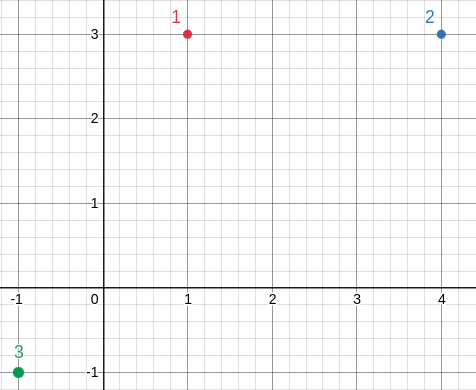
\includegraphics[scale=0.4]{graf.png}
		\captionof{figure}{The cities on the cartesian coordinate system}
		\label{fig:fig1}
	\end{minipage}
	\begin{minipage}{0.35\textwidth}
		\centering
		\begin{tabular}{|l|l|}
			\hline
			People who visited city \#$1$ & 3, 4 \\ \hline
			People who visited city \#$2$ & 2, 4 \\ \hline
			People who visited city \#$3$ & 3 \\ \hline
		\end{tabular}
		\captionof{figure}{People who visited each city}
		\label{fig:fig2}
	\end{minipage}
\end{figure}
The distance between cities \#$1$ and \#$2$ is $\sqrt{(1-4)^2 + (3-3)^2} = \sqrt{9} = 3$ (also the smallest).
The distance between cities \#$1$ and \#$3$ is $\sqrt{(1+1)^2 + (3+1)^2} = \sqrt{20} \approx 4.472135955$, whose floor is 4.

The people \#$1$ and \#$4$ don't have any visited city in common (so do the people \#$2$ and \#$3$).
The people \#$2$ and \#$4$ have both visited the city \#$2$.

The following pairs of people don't have any visited city in common: [1, 2], [1, 3], [1, 4], [2, 3].

\pagebreak
\section*{Exercise 2 (70 points)}
We have a rather barebones Svelte social media app, based on some \textit{hot} blockchain technology, that stores our posts and some various useful informations about the post.
You are tasked with adding some features to this app. More specifically:
\begin{itemize}
	\item Show the creation date of each post.
	\item Show the user towards whom each post was dedicated (if any). When the name is clicked, the person's profile page should appear.
	\item Let the user dedicate to someone in their friends list a post in the "Add post" interface.
	\item Show the amount of posts hooked to each post (if any), and let the user hook to a certain post by clicking a button (or whatever) nearby the post.
	\item If a post is hooked to an other post, show this, and let the user see the post being hooked to.
	\item Create a new feed tab with the posts dedicated towards our user, and an other one with the ones hooked to other posts by our user. Name them creatively.
\end{itemize}

Our app has good documentation and a good test coverage, so feel free to read the docs and apply them to your app, and also write good documantation and provide good test coverage for the code you write!
\subsection*{Procedure}
You shall clone in your workstation the git repository at \verb|https://10.192.192.19/ex2_|\fbox{ID}\verb|.git|, where \fbox{ID} is your given contestant ID.
There you should find our barebones app, that you will have to change to add the desired features.
Whenever you feel like it, you can push it in the remote.
This will trigger our CI to evaluate your sollution, and tell you in the terminal right after pushing it if there are any mistakes.
Your final submission shouldn't have any, otherwise it won't be valid.
After the time's up, you'll no longer be able to push your app in the remote, and we'll start manually evaluating it.
Note that \textbf{you only have available 50 CI runs for this problem}.
When they're all consumed, you won't be able anymore to see whether your app is failing the CI tests or not.
\end{document}

